\chapter{Dronetag web infrastructure}\label{ch:dronetag-web-infrastructure}
This chapter describes all Dronetag web infrastructure and contains a detailed description of the web Dronetag platform.
It consists of the all technical stack that ensures data providing.
We had to determine a convenient and reliable way of how to construct a useful architecture of infrastructure gradually.
It starts with an IoT module and frontend web client written in JavaScript, and it continues to implement WebSockets with alone Live Service based on a Kubernetes cluster.
Current parts of the stack are the following:
\begin{itemize}
    \item Load Balancer,
    \item OLP Message Broker,
    \item Message Queue,
    \item Backend,
    \item Frontend,
    \item Private API endpoint,
    \item Public API endpoint,
    \item Database Storage and
    \item Live Service.
\end{itemize}
The components and their relations are showed on the infrastructure diagram~\ref{fig:infrastracture-diagram}.
I must note the stack is being still involved anytime when we find out it is insufficient and complexity of the all system increasing.

\section{API separation}\label{sec:api-separation}
Due to security reasons, the web API divides into \textbf{Private} and \textbf{Public API} endpoints.
\textbf{Public API} is allowed to use by third-party consumers.

In further determination, this infrastructure divides into the \textbf{Staging} and \textbf{Production} environment.
Staging is for development and testing purposes, and it usually runs on the same version as Production.
Production is like a mirror of Staging.
The difference is that the Production environment contains a previous version of the software that is released.

\section{Docker deployment}\label{sec:docker-deployment}
Every web application in the stack is deployed and managed by \textbf{Docker}.
It is the easiest way to develop and publish new version software.
However, in the beginning, let us clarify what the Docker is.
"Docker is a tool designed to make it easier to create, deploy, and run applications by using containers.
Containers allow a developer to package up an application with all of the parts it needs, such as libraries and other dependencies, and deploy it as one package.
By doing so, thanks to the container, the developer can rest assured that the application will run on any other Linux machine regardless of any customized settings that machine might have that could differ from the machine used for writing and testing the code."\cite{dockerDescription}

To read about what a Container is and how useful it can be for business and can see on their official websites~\cite{dockerContainer} or here~\cite{dockerDescription}.

Thanks to the \textbf{Docker Compose} tool, we can have separated parts of the infrastructure.
In the case of more significant changes, we have to change only one module, and others are without changes.
In a nutshell, we have more containers that each of them contains individual responsibility for their processing, and \textbf{Docker Compose} joins them together.
If I simplify it, \textbf{Docker Compose} works like a composer that takes separate containers, where each of them can launch different technologies and compose it together into one whole infrastructure.\cite{dockerCompose}


\section{Kubernetes}\label{sec:kubernetes}
"Kubernetes (K8s) is an open-source system for automating deployment, scaling, and management of containerized applications."~\cite{kubernetes}
It means that Kubernetes is a tool allowing a running cluster whose single nodes may be as Docker containers.
This approach ensures scalability, whereas the number of Docker containers can be huge and can be created and disposed of dynamically based on the loading.
The advantage of Kubernetes is that it can detect a note out of order and initialize and deploy a new one to stay the optimal performance

"It groups containers that make up an application into logical units for easy management and discovery.
Kubernetes builds upon \textit{15 years of experience of running production workloads at Google}~\cite{kubernetesArticle}, combined with best-of-breed ideas and practices from the community."~\cite{kubernetes}
Thanks to these experiences, Kubernetes is a fine grain, and the cluster hierarchy is merely maintainable.

"Though widespread interest in software containers is a relatively recent phenomenon, at Google we have been managing Linux containers at scale for more than ten years and built three different container-management systems in that time."~\cite{kubernetesArticle}
How you can see, the idea of containerization has a rich history.
However, there were Linux Containers before the Docker ones.
That is the reason why we use it for web development.
It is easy to scale, maintain, and able to deploy to Google Cloud Platform.

\section{Backend application}\label{sec:backend-application}
Python Django Web API app %TODO


\section{Database model}\label{sec:database-model}
There is a database model figure in Dronetag backend.
The database model consists followings entities:
\begin{itemize}
    \item User,
    \item Aircraft,
    \item Device,
    \item Flight,
    \item Telemetry measurement,
    \item Organization,
    \item Fleet,
    \item Aircraft vendor,
    \item Aircraft model,
    \item Airspace zone,
    \item User preference and
    \item Organization preference.
\end{itemize}
A detailed diagram with relationships between entities is in the ERD Diagram of infrastructure in this picture.%\cite{fig:erd-diagram}

\subsection{User}\label{subsec:user}
This entity represents a user who signs up and logs in to the application.
...

All attributes are described like this:
\begin{itemize}
    \item id - represents the unique object identificator,
    \item email - represents ...
    \item full\_name - represents
    \item password\_hash - represents
    \item phone\_number - represents
    \item deleted - represents
    \item date\_created - represents
    \item data\_modified - represents
    \item last\_login - represents
    \item active - represents
    \item country - represents
\end{itemize}

\subsection{Aircraft}\label{subsec:aircraft}
This entity represents an aircraft that is connect with a Dronetag device.
...

All attributes are described like this:
\begin{itemize}
    \item id - represents the unique object identificator,
    \item name - represents an aircraft name for easier recognition in My aircraft list,
    \item uas\_operator\_id - represents a unique code identifying a pilot who registered this aircraft,
    \item weight - represents a weight of the aircraft,
    \item date\_created - represents a date when was an aircraft added,
    \item data\_modified - represents a date when was an aircraft changed,
    \item deleted - represents a date when was an aircraft deleted.
\end{itemize}

\subsection{Device}\label{subsec:device}
This entity represents a physical device that sends live information to the Dronetag platform.
...

All attributes are described like this:
\begin{itemize}
    \item id - represents the unique object identificator,
    \item serial\_number - represents ...
    \item name - represents
    \item type - represents
    \item comm\_id - represents
    \item date\_created - represents
    \item date\_modified - represents
    \item last\_battery - represents
    \item last\_rsrp - represents
    \item last\_message - represents
\end{itemize}

\subsection{Flight}\label{subsec:flight}
This entity represents it represents a flight that a user has created.
...

All attributes are described like this:
\begin{itemize}
    \item id - represents the unique object identificator,
    \item date\_planned\_start - represents ...
    \item date\_planned\_finish - represents ...
    \item date\_started - represents ...
    \item date\_finished - represents ...
    \item status - represents
    \item distance - represents
    \item duration - represents
    \item region\_geojson - represents
    \item max\_flight\_altitude - represents
    \item takeoff\_latitude - represents
    \item takeoff\_longitude - represents
    \item takeoff\_geo\_alt - represents
    \item takeoff\_pressure - represents
    \item public - represents
    \item date\_created - represents
    \item date\_modified - represents
    \item deleted - represents
\end{itemize}

\subsection{Telemetry measurement}\label{subsec:telemetry-measurement}
This entity represents a ...

All attributes are described like this:
\begin{itemize}
    \item time\_received - represents the unique object identificator,
    \item time - represents ...
    \item latitude - represents
    \item longitude - represents
    \item altitude - represents
    \item geo\_altitude - represents
    \item velocity\_x - represents
    \item velocity\_y - represents
    \item velocity\_z - represents
    \item gnss\_accuracy - represents
\end{itemize}

\subsection{Organization}\label{subsec:organization}
This entity represents a ...

All attributes are described like this:
\begin{itemize}
    \item id - represents the unique object identificator,
    \item name - represents ...
    \item description - represents
    \item date\_created - represents
    \item date\_modified - represents
    \item deleted - represents
\end{itemize}

\subsection{Fleet}\label{subsec:fleet}
This entity represents a ...

All attributes are described like this:
\begin{itemize}
    \item id - represents the unique object identificator,
    \item name - represents ...
    \item color - represents
    \item deleted - represents
    \item date\_created - represents
    \item date\_modified - represents
\end{itemize}

\subsection{Aircraft vendor}\label{subsec:aircraft-vendor}
This entity represents a ...

All attributes are described like this:
\begin{itemize}
    \item id - represents the unique object identificator,
    \item name - represents a vendor name.
\end{itemize}

\subsection{Aircraft model}\label{subsec:aircraft-model}
This entity represents a user who signs up and logs in to the application.
...

All attributes are described like this:
\begin{itemize}
    \item id - represents the unique object identificator,
    \item name - represents ...
    \item weight - represents
    \item vendor\_id - represents a relationship to a Vendor.
\end{itemize}

\subsection{Airspace zone}\label{subsec:airspace-zone}
This entity represents a ...

All attributes are described like this:
\begin{itemize}
    \item id - represents the unique object identificator,
    \item name - represents ...
    \item country - represents
    \item region\_geojson - represents
    \item date\_created - represents
    \item date\_modified - represents
\end{itemize}

\subsection{User preference}\label{subsec:user-preference}
This entity represents a ...

All attributes are described like this:
\begin{itemize}
    \item property - represents ...
    \item value - represents ...
    \item date\_modified - represents
\end{itemize}

\subsection{Organization preference}\label{subsec:organization-preference}
This entity represents a user who signs up and logs in to the application.
...

All attributes are described like this:
\begin{itemize}
    \item property - represents the unique object identificator,
    \item value - represents ...
    \item date\_modified - represents
\end{itemize}

\begin{figure}
    \centering
    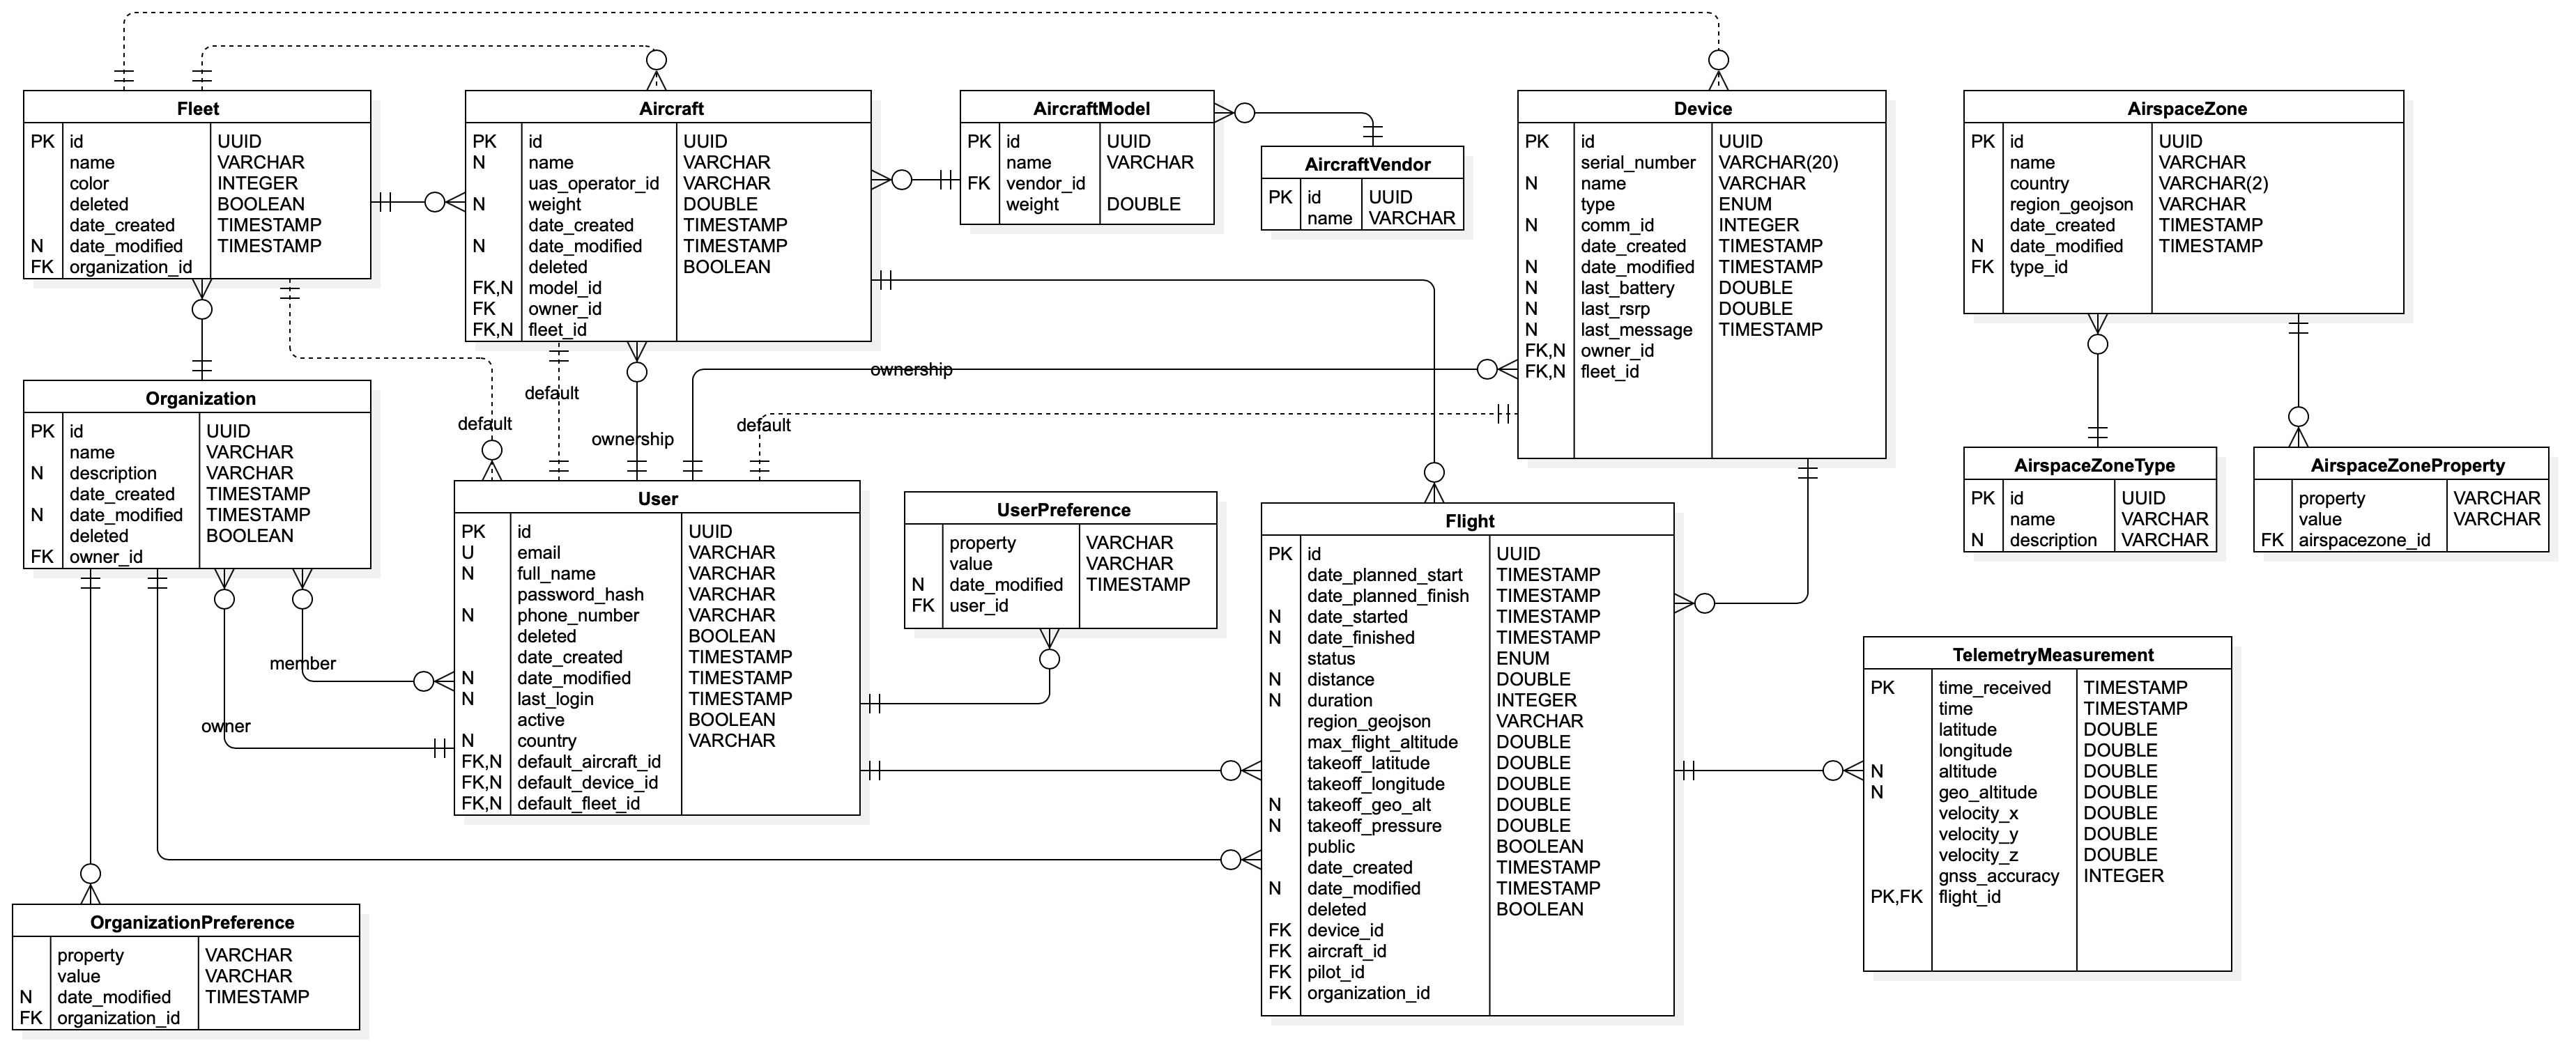
\includegraphics[scale=0.31, angle=90]{assets/erd_diagram.png}
    \caption{ERD Diagram of data model\cite{dataModel}}
    \label{fig:erd-diagram}
\end{figure}

\subsection{Live Service database model}\label{subsec:live-service-database-model}
In additional, during the development we had found out the current backend is not sufficient for our needs, so we decided to divide the backend model into backend one and Live Service model.
Because there are only live real time temporary data, so we deployed a Redis database.

"Redis is an open source (BSD licensed), in-memory data structure store, used as a database, cache and message broker.
It supports data structures such as strings, hashes, lists, sets, sorted sets with range queries, bitmaps, hyperloglogs, geospatial indexes with radius queries and streams.
Redis has built-in replication, Lua scripting, LRU eviction, transactions and different levels of on-disk persistence, and provides high availability via Redis Sentinel and automatic partitioning with Redis Cluster."\cite{redis}
It means that the Redis is a real-time storage that persists data only for very short time.
That is the reason, why it is suitable for this purpose.

The Live Service database model consists of \textbf{Device} and \textbf{Telemetry} entity.



\section {Broker}\label{sec:broker}


\section{Communication protocols}\label{sec:communication-protocols}
The communication protocols in Dronetag infrastructure are the following:
\begin{itemize}
    \item OLP Protocol,
    \item AMQP (Advanced Message Queuing Protocol) and
    \item HTTP(S) REST.\cite{dataInfrastructure}
\end{itemize}

\subsection{OLP Protocol}\label{subsec:olp-protocol}
OLP messages flow between Dronetag devices and a web platform.
It is about binary messages that are transfer by UDP packets.\cite{dataInfrastructure}

\subsection{Advanced Message Queuing Protocol}\label{subsec:advanced-message-queuing-protocol}
Advanced Message Queuing Protocol is for communication with a message queue.
It wraps Celery.\cite{dataInfrastructure}

\subsection{HTTP(S) REST}\label{subsec:httpnullsnullrest}
Clients' applications communicate to a server to fetch data from the platform via HTTPS protocol with REST architecture.\cite{dataInfrastructure}


\begin{figure}
    \centering
    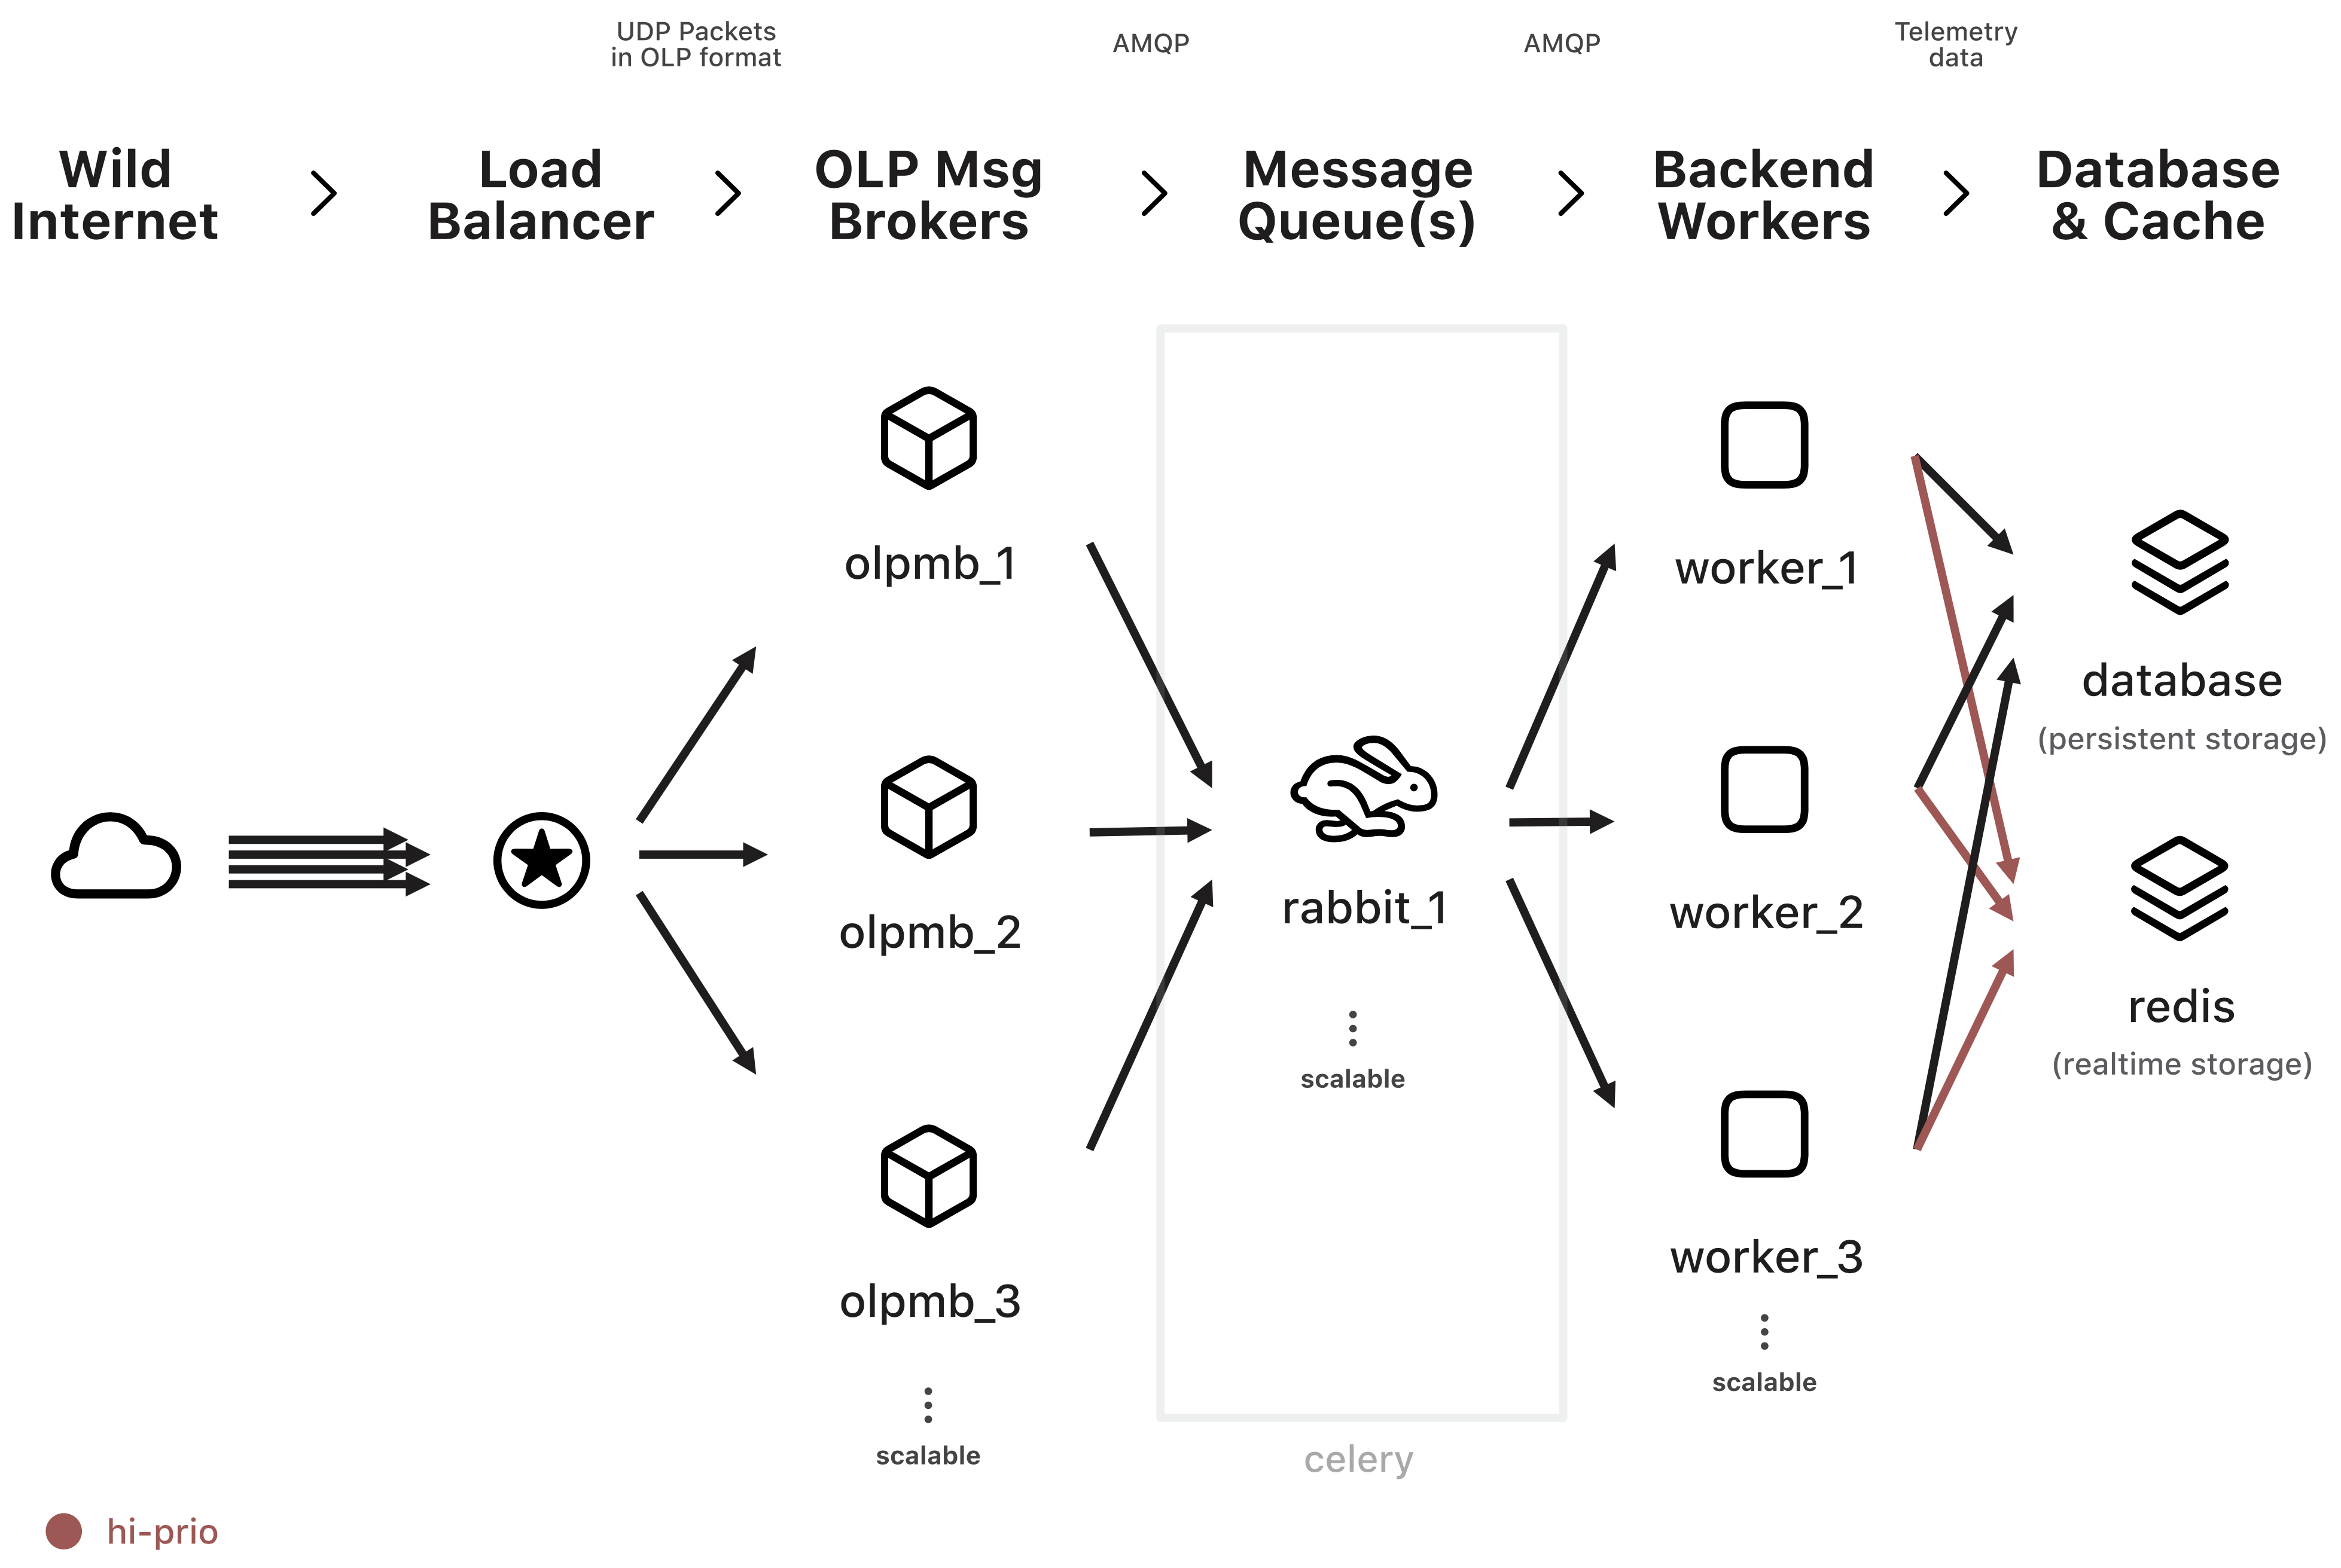
\includegraphics[scale=0.29, angle=90]{assets/infrastructure-diagram.png}
    \caption{Infrastructure diagram~\cite{dataInfrastructure}}
    \label{fig:infrastracture-diagram}
\end{figure}
